%\thispagestyle{myheadings}
\section{Invited Talk: Gina R Kuperberg}
\index{Kuperberg, Gina R}
\begin{center}
%% --- Keynote Address ---
%% \vspace{2em}\\
%% \vfill

\begin{Large}
{\bfseries\Large ``Predicting Meaning: What the Brain tells us about the Architecture of Language Comprehension''}\vspace{1em}\par
\end{Large}

{\itshape Gina R. Kuperberg}\vspace{1em}\par
Monday, June 10, 2013, 9:00am -- 10:10am \vspace{1em}\\
\index{Kuperberg, Gina R.}
\PlenaryLoc \\
\vspace{1em}\par 
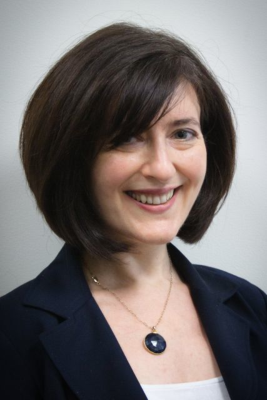
\includegraphics[height=100px]{content/day2/kuperberg-headshot.pdf}
\end{center}

\noindent
{\bfseries Abstract:} It is well established that we draw upon our real-world knowledge to predict
upcoming events and even individual words. I will discuss evidence that the neurocognitive
mechanisms that we engage in retrieving conceptual information associated with incoming words are
quite distinct from those engaged when these predictions are disconfirmed by the input. Drawing
broad links with computational models conceptualizing language comprehension as an incremental
process of belief updating, I will suggest that the engagement of these distinct neurocognitive
systems allows for comprehension that is both highly efficient and highly flexible (1).

I will first discuss studies using event-related potentials (ERPs) to examine online brain activity
during sentence and discourse comprehension. I will then draw some (still tentative) links between
this ERP literature and some relevant fMRI and MEG studies. Finally, I will discuss the advantages
of a predictive comprehension system. Predicting correctly clearly offers advantages in terms of
computational efficiency. Here I will argue that the costs incurred when we predict incorrectly are
also crucial for successful and flexible comprehension. Neurocognitive responses triggered by
prediction errors may rescue us from interpretation errors in noisy environments, may allow us learn
novel events, and may enable us to flexibly adjust our comprehension strategies in response to
everchanging task and environmental demands.

\vspace{3em}\par 

\vfill
\noindent
{\bfseries Biography}: Gina R Kuperberg is a Cognitive Neuroscientist and a Professor in the
Department of Psychology and the Cognitive Science Center at Tufts University, Boston. She is also a
Board Certified Psychiatrist and a Principal Investigator in the Psychiatry Neuroscience Program at
Massachusetts General Hospital, Harvard Medical School. Her research program aims to understand the
neurocognitive mechanisms by which the human brain builds meaning from language, and how these
mechanisms break down in neuropsychiatric disorders, particularly schizophrenia.

Dr.\ Kuperberg's Lab is situated across in both the Department of Psychology at Tufts and the
Martinos Center for Biomedical Imaging at Massachusetts General Hospital. The Lab uses multimodal
neuroimaging methods –– event-related potentials (ERPs), functional MRI (fMRI) and
magneto-encephalography (MEG) –– to probe both the spatial and temporal dimensions of cognition in
the brain. Her research program is funded by an RO1 from the National Institute of Mental Health
(NIMH), as well as awards from the Brain and Behavior Research Foundation and the Sidney Baer
Trust. She, her students, postdocs and collaborators publish in a wide range of journals of
Cognitive Neuroscience, Psycholinguistics, Experimental Psychology, Neuroimaging and Psychiatry.

Dr.\ Kuperberg has served as a standing member for the Language and Communication Study Section for
the National Institute of Health, and as a committee representative for Language for the Cognitive
Neuroscience society. Her research accomplishments have been recognized by several awards, including
the A.E. Bennett Research Award from the Society for Biological Psychiatry, the Joseph Zubin Award
for Significant Contributions to Research in Psychopathology, and an Award from Brain Research for
their most highly cited article, for her review of the architecture of the language system, Neural
Mechanisms of Language Comprehension: Challenges to Syntax.

Dr.\ Kuperberg earned her MD at St. Bartholomew's Medical School, London, and her PhD in Psychology
and Cognitive Neuroscience at Kings College, University of London. She completed an internship at
St. Bartholomew's Hospital and residency training in Psychiatry at the Maudsley Hospital and
Institute of Psychiatry, London. In 1998, she came to Boston where she completed research
fellowships in Neuroimaging and Cognitive Electrophysiology at Massachusetts General Hospital,
Harvard Medical School and Tufts University, working with David Caplan, Anders Dale and Phil
Holcomb.
\newpage
